% Submission to Scientific Programming: adapted from paper in ICCS2006,
% "Workflow systems in e-Science" workshop

% Changes from WSES workshop paper:
% * Reworked intro
% * More on security and (GSI)-SSH
% * Added section on running on Condor/SGE
% * Added two figures

\documentclass[a4paper]{article}

\usepackage{graphics}
\usepackage{setspace}

\usepackage{caption}
\usepackage{alltt}
\usepackage[left=40mm, right=40mm, top=40mm, bottom=40mm]{geometry}

% Make figures come out as "Fig. 1" instead of "Figure 1"
\renewcommand{\figurename}{Fig.}

% I tried to create a bibtex style file for Scientific Programming but didn't get it quite right...
%\bibliographystyle{plain}


\begin{document}
\doublespacing

\begin{center}
%TODO: change the title
{\Large Styx Grid Services: Lightweight Workflow Middleware for Grid Environments}

\bigskip
\bigskip

{\large J.D. Blower$^{1}$, A.B. Harrison$^{2}$ and K. Haines$^{1}$}

\bigskip

{\small 1. \textit{Reading e-Science Centre, Environmental Systems Science Centre, \\
University of Reading, Reading RG6 6AL, UK} \\
Email: \{jdb, kh\}@mail.nerc-essc.ac.uk\\
Tel: +44 (0)118 3788741 \\
\medskip
2. \textit{School of Computer Science, Cardiff University, Cardiff CF24 3AA, UK}\\
Email: a.b.harrison@cs.cardiff.ac.uk\\
Tel: +44 (0)29 20876964}

\bigskip
\bigskip

Keywords: Styx, streaming, third-party transfers, WS-RF, Condor, Globus

\end{center}

\newpage

\begin{abstract}
The service-oriented approach to performing distributed scientific research is potentially very powerful but is not yet widely used in many scientific fields.  This is partly due to the technical difficulties involved in creating services and workflows and the inefficiency of many workflow systems with regard to handling large datasets.  We present the Styx Grid Service, a simple system that wraps command-line programs and allows them to be run over the Internet exactly as if they were local programs.  Styx Grid Services are very easy to create and use and can be composed into powerful workflows with simple shell scripts or more sophisticated graphical tools.  An important feature of the system is that data can be streamed directly from service to service, significantly increasing the efficiency of workflows that use large data volumes.  The status and progress of Styx Grid Services can be monitored asynchronously using a mechanism that places very few demands on firewalls.  Styx Grid Services can interoperate with with Web Services and WS-Resources using suitable wrappers and brokers.
\end{abstract}

\section{Introduction}\label{sec:intro}
The use of service-oriented architectures (SOAs) in scientific computing is increasing.  The principal advantage of the SOA approach is that scientists can access resources such as databases, high-end computing resources, laboratory equipment and sensor networks over the Internet without knowledge of the underlying infrastructure.  Several independent services can be combined in a distributed application or \textit{workflow\/} to solve a particular problem.  For example, a scientist might wish to construct a workflow in which several pieces of data are extracted from databases in different locations, analyzed using a distributed computing resource, then finally visualized on his or her local machine.

At present, however, there are very few examples of scientific communities that work routinely in this way.  Part of the reason for this is that the creation of such services and workflows is beyond the technical expertise of most scientists, often due to the complexity of the required middleware~\cite{chin:2004}.  Furthermore, many workflow systems suffer from inherent limitations that are important in the scientific domain.  These vary from system to system but commonly include:

\begin{itemize}
\item A centralized data flow architecture: all data must pass through the workflow engine.
\item A focus on SOAP and XML as the data transport format.  It is very inefficient to encode anything other than a small amount of data in XML due to the processing time required and the inflating effect of doing so.  The use of SOAP attachments gives a smaller data size than XML but still requires data to be encoded and decoded~\cite{bustamente:2000, chiu:2002, davis:2002}.
\item A notification mechanism that requires the client to listen on incoming ports or to poll the server frequently.  This is discussed further in section~\ref{sec:notification} below.
\end{itemize}

We describe a service type that addresses the above issues: the \textit{Styx Grid Service} or SGS.  A Styx Grid Service is a service that wraps a command-line (i.e.\ non-graphical) program and allows it to be run remotely.  Styx Grid Services are very easy to create, deploy and use~\cite{blower_escience:2006, blower_lncs:2006, blower:2005} and can be composed into workflows using shell scripts or specialized workflow tools.  Workflows that are composed from Styx Grid Services work efficiently with large datasets: data are transported in their most compact binary form and can be streamed directly from service to service (a decentralized data flow architecture).  Through the use of wrappers and brokers, SGSs can interoperate with tools and services based on Web Services and the Web Services Resource Framework (WSRF~\cite{WSRF}).

The details of how Styx Grid Services are created and used from a user's point of view can be found in previous publications~\cite{blower_escience:2006, blower_lncs:2006, blower:2005} and the project website~\cite{sgswebsite}.  In this paper we shall focus on how the SGS system enables the creation of efficient scientific workflows. 

\section{Styx Grid Services: architecture}\label{sec:architecture}

The basis of the SGS system is the well-established Styx protocol for distributed systems~\cite{Pike:1999}.  Styx is a key component of the Inferno \cite{Inferno} and Plan~9 \cite{Plan9} operating systems (in Plan~9, Styx is known as ``9P'': the current version of Styx is equivalent to 9P2000).  In Inferno and Plan~9, applications communicate with all resources using Styx, without knowing whether the resources are local or remote.  Styx is essentially a file-sharing protocol, similar in some ways to NFS.  However, in a Styx system the ``files'' are not always literal files on a hard disk.  They can represent a block of RAM or the interface to a program, database or physical device.  Styx can therefore be used as a uniform interface to access diverse resource types.  Whereas in Remote Procedure Call (RPC)-style Web Services the resources are accessed through a set of methods, Styx resources are accessed by reading from and writing to a hierarchy of files, which is known as a \textit{namespace\/}.

A Styx Grid Service wraps a command-line executable and exposes it to the network as a namespace (virtual filesystem).  This namespace contains files that represent the input and output files of the executable and the command-line arguments.  It also contains files that allow the service to be controlled and monitored.  A full description of the SGS namespace is not given here for reasons of space: the reader is referred to the SGS website~\cite{sgswebsite} and previous publications~\cite{blower_escience:2006, blower_lncs:2006, blower:2005}.  A single SGS server can contain many SGSs and can service multiple clients simultaneously.  The server is configured through an XML file that defines each wrapped executable in terms of its inputs, outputs and arguments~\cite{blower_escience:2006}.

All files in the SGS namespace can be referenced by a unique URL.  For example, the file that represents the standard output stream of instance \texttt{1} of the the \texttt{mySGS} service can be identified by \texttt{styx://<server>:<port>/mySGS/instances/1/outputs/stdout}.  This is very important for workflows: these URLs are passed between services in a workflow as \textit{pointers to data}, to enable the direct transfer of data between services (see section~\ref{sec:datapassing}).

Styx clients typically maintain persistent connections with the server: this is important for asynchronous notification, as discussed in section~\ref{sec:notification} below.  We have developed a pure-Java implementation of the Styx protocol (JStyx~\cite{JStyx}) and we use this as the basis for the Styx Grid Services software.

In some respects, the SGS system is similar to the GriddLeS~\cite{abramson:2004} system.  Both systems TODO TODO TODO : both work with unmodified executables, except that SGS wraps executables, GriddLeS intercepts local I/O calls and redirects them to the network at run time.  GriddLeS also handles replica file systems etc.  However, GriddLeS cannot redirect standard streams (CHECK THIS).

\subsection{Asynchronous notification}\label{sec:notification}
With long-running services it is desirable for clients to be able to monitor the progress and status of the remote service.  Many notification systems (e.g.\ WSRF) employ methods whereby either (i) the client runs a server process that listens for messages or (ii) the client polls the server at intervals for updates.  Method (i) will be defeated if the client is behind a stringent firewall or NAT system and method (ii) can be inefficient, leading to the client and server exchanging many redundant messages.

In the SGS system the problem is solved in the following way.  The client makes a persistent connection with the server and reads from a particular file in the SGS namespace to get a piece of status information.  Having received the reply, the client immediately sends a message to read from the same file.  The server will not respond to this message until the status information has changed.  This is permitted by the design of the Styx protocol, which allows read requests and their reponses to be decoupled.

\subsection{Data transfers in Styx}\label{sec:datatransfer}
It is important to understand how bulk data are transferred in the Styx protocol.  When a client downloads data from a Styx server it does so in chunks: it sends read requests for individual chunks of typically 8KB in size.  When the server replies with the data the client sends another read message and so forth.  This method is to allow a single socket connection to be used for multiple simultaneous tasks (data transfer, progress monitoring, etc.) but leads to less efficient bulk transfer than, for example, HTTP.  The throughput of data can be increased by (i) increasing the chunk size and (ii) sending multiple read requests without waiting for a reply.  By combining these two methods we have found it possible to achieve 95\% of HTTP transfer rates~\cite{blower:2004}.

\subsection{Direct data streaming}\label{sec:datapassing}
A very important feature of the SGS system is that it allows workflows to be constructed in which data are passed \textit{directly} from service to service in their most efficient binary form.  To explain how this works, let us consider a workflow of two Styx Grid Services, A and B, in which output data from A must be sent directly to B, without passing through the workflow engine.

\begin{enumerate}
\item The workflow engine creates a new instance of service A and starts it.
\item Instead of downloading the output from service A, the workflow engine obtains a \textit{reference} to the output file or stream.  This reference is the URL of the relevant virtual file in the namespace of service A.
\item The workflow engine creates a new instance of service B.
\item Instead of uploading an input file to service B, the workflow engine uploads the reference to the output of service A.
\item The workflow engine starts service B.  Service B downloads the data from service A and passes it to the underlying executable, either as a regular input file or on the standard input stream of the executable.
\end{enumerate}

There are two important things to note about this mechanism.  Firstly, data are \textit{pulled} from service B, not pushed from service A.  Secondly, any number of other services or clients could download the output from service A giving the effect of forking the data stream between multiple services.  The SGS server maintains a cache of all output files, allowing multiple clients to download data from different portions of the file.  In this way, even the standard streams of a program can be made to be seekable, and thus treated identically to regular files.

The chunked method of data transfer (section~\ref{sec:datatransfer}) ensures that there can be no problems with buffer over- or under-runs due to a slow data consumer being overwhelmed with data from a fast producer.  A data consumer will only request a data chunk when the consumer is ready (preventing over-runs): conversely a server will not reply to a data request until the data are available (preventing under-runs).

\subsection{Security}
SGS servers can be secured in more than one way.  A server can execute as a persistent daemon with its own user database and authentication protocol and traffic can be optionally encrypted using a Secure Sockets Layer.  Alternatively, the server can be executed through the Secure Shell (SSH), using the SSH authentication mechanism and secure channels.  The use of SSH and SGS in combination allows the fast creation of cross-institutional Grids without requiring heavyweight middleware solutions or the opening of a large number of firewall holes.  A discussion of the relative merits of these approaches to securing the SGS system is outside the scope of this paper but further details can be found in~\cite{blower_escience:2006}. 

\subsection{Integration with other Grid resources}
The SGS system can be employed as an easy-to-use front end to Distributed Resource Managers such as Condor~\cite{condor}, Sun GridEngine~\cite{sungridengine} and Globus~\cite{globustoolkit}.  The SGS server exposes the same namespace in all cases and so no change to client software is needed.  In these cases, jobs are not run on the SGS server itself, but on a set of distributed resources such as a cycle-stealing pool of desktop machines or a compute cluster.  For more details the reader is referred to~\cite{blower_escience:2006}.

\section{Workflow case study}\label{sec:casestudy}
In order to illustrate the above concepts we shall describe a particular data-intensive workflow that is particularly suited to the SGS approach.  In the environmental sciences, computer models of atmospheric and oceanic circulation are driven and validated by observations.  The science of \textit{data assimilation} is concerned with the process of combining these observations with numerical models in order to increase the predictive skill of the model.  In data assimilation it is important to know how certain quantities are correlated with each other and with themselves over time~\cite{haines:2006}).  In the context of an ocean circulation model, a \textit{one-point correlation map} displays how the evolution of a certain quantity, such as the salinity on the 12$^\circ$C isotherm, at a single point correlates with the evolution of the same quantity at its neighbouring points in the model.  This gives a characteristic length scale for key physical processes.

In one such investigation~\cite{haines:2006}, we constructed a workflow of three Styx Grid Services.  The first service (\texttt{extract}) extracts data from an archive and outputs it as a set of timeseries.  The second service (\texttt{filter}) filters the data by removing the signal of the seasonal cycle, which would otherwise dominate the data.  The third service (\texttt{calcCorrelation}) calculates the one-point correlation map from the filtered data.

The executables that underlie the SGSs are simple C programs that read data from their standard input stream and output data to the standard output stream.  Therefore, if they were running on the same machine, the whole calculation could be performed by running:

\texttt{extract <params> $|$ filter $|$ calcCorrelation}

\noindent where \texttt{<params>} are the parameters of the extraction process, which do not concern us here.  Note that, through the use of the \texttt{SGSRun} client program (see section~\ref{sec:sgsrun} below), the above calculation can be run as a workflow over a set of distributed services with exactly the same command line~\cite{blower_lncs:2006}.  Each service deals with approximately 24MB of binary data, which is far too large to consider encoding as XML, or even as SOAP attachments: the resulting process would be very inefficient.

The conceptual workflow, with an example result, is shown in Figure~\ref{fig:workflow}.  This workflow is particularly suited to a data streaming approach because the downstream services (\texttt{filter} and \texttt{calcCorrelation}) can begin their work before all the data is extracted by the \texttt{extract} service.  Close analogues of this process can be found in many scientific fields such as signal processing.

\subsection{Timing tests}
The simple workflow of three SGSs can be constructed in four different ways.  The workflow can either pass data directly between the services, or the data can be passed through the workflow engine.  Additionally, the workflow can either execute the service sequentially (i.e.\ the \texttt{extract} service must complete before the \texttt{filter} service can start, and so forth) or concurrently, in which all three services can run simultaneously on a continuous data stream.

The results of the four different possibilities are shown in figure~\ref{fig:workflowspeeds}.  As expected, the most efficient case is the one in which data are streamed directly from service to service and in which the three services execute concurrently.

Although the direct data streaming approach is clearly the most efficient in this case, a similar increase in efficiency will not always be seen in other workflows.  If, for example, a workflow is dominated by a slow-running service, the increase in data transfer efficiency might not have a large effect on the overall execution time.  However, for data-intensive workflows, particularly where the workflow engine (i.e.\ the client) has a low-bandwidth connection to the service hosts, the advantage to the direct streaming approach is likely to be marked.  Not all services will support streaming: in many cases the services in a workflow will execute sequentially.  However, figure~\ref{fig:workflowspeeds} shows that there is still a distinct advantage to passing the data directly between the services.


\section{Interfaces to Styx Grid Services}\label{sec:interfaces}

The above discussion and results are independent of the choice of workflow engine.  There are many ways for a client to interact with Styx Grid Services and create workflows from them.

\subsection{Command-line interface}\label{sec:sgsrun}
The \texttt{SGSRun} program, which is distributed with the SGS software, is a generic command-line client program for any SGS.  It allows remote SGSs to be run \textit{exactly as if they were local programs}~\cite{blower_lncs:2006, blower_escience:2006}.  Input/output files are automatically uploaded/downloaded and command-line parameters are parsed.  Through the \texttt{SGSRun} program, simple workflows can be created with shell scripts.  This is perhaps the simplest way of creating SGS workflows.

\subsection{Graphical workflow tools}\label{subsec:graphical-workflow}
In some cases, there are significant advantages in using more sophisticated graphical tools to interact with services and create workflows.  In particular, graphical interfaces can provide richer interactivity with the SGS server: progress and status can be monitored graphically, input parameters can be set using graphical controls and the service can be steered~\cite{blower:2005}. Furthermore, to provide greater interoperability with other Grid environments it can be advantageous to wrap SGS in standards compliant interfaces using ubiquitous protocols such as HTTP. In the following subsections we describe current bindings to SGS in other systems.

The Taverna workbench (\texttt{http://taverna.sf.net}) is a graphical workflow system that was designed for performing {\it in silico} experiments in the field of bioinformatics, but it is sufficiently general to be useful to other communities.  We have worked with the Taverna developers to incorporate support for Styx Grid Services into the software.  Using Taverna, the user can build workflows by mixing diverse service types, including Web Services and SGSs.

The Triana workflow system (\texttt{http://trianacode.org}) is a graphical workflow environment that can interface with many different service types but cannot currently interface directly with Styx Grid Services.  As a result we have developed two ways of achieving integration using Web services which are supported in Triana. The first mechanism uses a brokered architecture, in which a separate Web Service is created that accepts SOAP messages and uses the information therein to communicate with an SGS server. This is described in more detail in~\cite{blower:2005}.

The second mechanism uses WSPeer~\cite{wspeer}, the Peer-to-Peer oriented Web Service framework that is used by Triana. WSPeer has a binding to the Styx protocol for delivering SOAP messages over Styx. This allows the Styx Grid Service itself to accept SOAP messages that are written directly to a file in its namespace.  When the SGS is deployed using WSPeer, a WSDL~\cite{WSDL} document is generated and placed into the SGS namespace so it can be read by clients. This WSDL document defines service operations that encapsulate the messages and data to be written to the files in the SGS namespace. For example, the WSDL will contain an operation for setting the input to the SGS which might have a signature such as  \texttt{setStdin(String url)}. To tell the SGS to read its input data from a particular URL, a client can invoke the operation. 

\subsection{Wrapping SGSs as WS-Resources}\label{subsec:ws-resources}

The Web Services Resource Framework (WSRF) is a recent specification which addresses the need to handle network exposed entities that maintain state across multiple service invocations. Styx Grid Services fall into this category because they display stateful characteristics -- they are created, have a lifetime, and have available properties such as the current status of the wrapped program. WS-RF uses the \textit{WS-Resource} abstraction to represent resources that are exposed and manipulated via a Web Service. A WS-Resource contains a service endpoint and a resource identifier. A client with a suitable WS-Resource can invoke the service at the endpoint specified and decorate the SOAP header of the request with the resource identifier. The service maps the identifier to some back-end resource -- in our case an SGS instance -- and invokes the requested operation on the resource.

WSPeer supports WSRF and can be used to expose an SGS as a WS-Resource. This is achieved by transforming the SGS configuration information (see section~\ref{sec:architecture}) into \textit{ResourceProperties\/}. These are QName/value pairs of a specified data type that are used to describe a WS-Resource type in the service WSDL as an XML schema element. Therefore a service that is being deployed as a front-end to an SGS will parse this configuration file for any program specific parameters and combine this with the standard SGS properties that are represented in the namespace. These properties are used to populate an XML schema element which is a template of the particular SGS type, and is inserted into the service WSDL. Service clients can read this schema to determine the available properties of an SGS.

There are a number of synergies between the WSRF suite of specifications and the properties defined by an SGS. For example, the \texttt{time/} directory in the SGS namespace, which houses files containing data pertinent to the lifetime of the service, can be mapped onto the properties defined in the WS-ResourceLifetime~\cite{wsrf-lifetime} specification. Likewise the \texttt{serviceData/} directory of the SGS namespace contains state data which are easily mapped to ResourceProperties or can be exposed as WS-Notification~\cite{wsrf-notification} topics that clients can subscribe to and receive notifications of changes from.

WSPeer is capable of wrapping an SGS as a WS-Resource in two ways.  The first way (brokering) involves creating a WSRF service that receives SOAP messages over HTTP and translates the information therein into Styx messages, which it sends to a separate SGS server (which may be on the same host). The second is to use the Styx protocol itself to send and receive XML. In this case the WSRF service that is exposing the SGS as WS-Resources is deployed at a Styx endpoint. The ability of WSPeer to use the Styx protocol directly allows clients that are behind firewalls and NAT systems to receive WS-Notification messages via the notification mechanism described in section~\ref{sec:notification}, thus overcoming the problem of clients needing to provide an accessible network address to receive notifications.

While it is useful to expose SGS functionality according standard specifications, we do not attempt to wrap the SGS data streams in XML for performance reasons. For example, an output stream exposed as a ResourceProperty consists of a URI from which data can be received. However, the actual data in the stream is application specific.


\section{Related work}\label{sec:related}

A number of systems are addressing the need to support data streaming in a variety of domains. In~\cite{brettlecker:2004}, the authors extend the OSIRIS~\cite{schuler:2003} system to enable data stream processing in the field of healthcare. The data stream management sub-system is constructed from a Peer-to-Peer network of \emph{Operators} deployed on a varity of devices including sensors, that accept, transform and output data streams. Different classes of Operators perform different transformations (e.g.\ noise reduction). Special Web Service Operators interface to the outside world allowing data to be stored or rendered remotely as well as control parameters to be passed into the network of Operators. The concept of Operators is similar to the use of pipes in SGS. While work on SGS has focussed on wrapping legacy applications for use on Grids, the Styx protocol is well suited to deployment in lightweight environments due to its low overhead and was originally specifically designed with resource-constrained devices in mind. The application of SGS to these environments is a focus of future research.

In~\cite{bioernstad:2006} the authors address the limitations of business process modeling techniques in handling data streams. The research focusses on how to manage state transitions within workflow components based on traditional request/response style interactions, specifically how to enable iterative re-execution of a component as a result of receiving data streams. SGS is does not limit itself to business process modeling techniques. This gives the architecture flexibility although it does place the burden of understanding the behavior of workflow components on the workflow designer.

In the context of Grid computing data streaming is being addressed with regard to several fields including geospatial data and astronomical data processing. The Cactus Computational Toolkit~\cite{allen:2001} has supported streaming for a number of years, specifically for remote visualization purposes, including the ability to stream to multiple clients simultaneously. In~\cite{fox:2006}, the authors present data streaming services based on the NaradaBrokering~\cite{naradabrokering} messaging system. Services are presented that stream GPS data from sensors as well as services that extend the capabilities of the Open Geospatial Consortium (OGC) data services to provide streaming of time-dependent data. The authors note the inefficiency of SOAP and provide data filters to transform streamed data. Similar to the WSRF/SGS intergation, the system uses SOAP for negotiation and optimized binary encoding for data transfer. A similar approach is taken by the UniGrids Streaming Framework~\cite{benedyczak:2006}. Here, like the WSRF/SGS integration, WSRF is used specifically to control and monitor the lifetime and parameters of optimized data streams. The AstroGrid-D~\cite{astrogrid-d} project is currently designing a data stream management system for handling astronomical data. Again it uses WSRF, and like the NaradaBrokering example uses the publish/subscribe pattern for receiving streams. The WSRF binding to SGS also allows notification of SGS property changes.

\section{Discussion}

We have described a new type of Internet service, the Styx Grid Service (SGS).  SGSs wrap command-line programs and allow them to be run from anywhere on the Internet exactly as if they were local programs.  SGSs can be combined into workflows using simple shell scripts or more sophisticated graphical workflow engines.  Data can be streamed directly between SGS instances, allowing workflows to be maximally efficient.  We have shown that Styx Grid Services can operate as part of a Web Services or WSRF system through the use of methods including broker services.

The SGS system has some important limitations:

\begin{itemize}
	\item The entities that are passed between services in a workflow are files and are not typed.  There is no way for the workflow enactor (e.g.\ a shell script) to tell whether the type of the output from one service matches the type of the input of the next service.  It is up to the services themselves to check that their inputs are valid.
	\item Although constructs such as loops are supported by the shell scripting interface (and graphical workflow tools), the variables used to control these loops cannot be read directly from the outputs of SGSs.
	\item Data transfer rates between services through the Styx protocol are slower than through HTTP or GridFTP~\cite{blower:2005}.  The SGS system may therefore not be optimal for problems that involve very large file transfers.
\end{itemize}

An important subject of future research would be to use the SGS approach to wrap entities such as classes and functions, rather than whole executables: in this case, inputs and outputs could be strongly typed and could also be captured by workflow engines, solving some of the above problems.

The SGS system has been designed so that services and workflows are easy to create.  It is well within the reach of most end-users (scientists) to do so with no help from dedicated technical staff.  Problems connected with firewalls and NAT routers are vastly reduced compared with other systems, allowing for easy deployment and use.  Large datasets are handled efficiently.  We believe that the Styx Grid Services system represents a significant step forward in increasing the usability and performance of service-oriented systems and workflows in science.
%

\section*{Acknowledgements}
The authors would like to thank Tom Oinn for incorporating the SGS framework into Taverna, Vita Nuova Holdings Ltd.\ for technical help with the Styx protocol and three anonymous reviewers for helpful comments.  This work was supported by EPSRC and NERC, grant refs. GR/S27160/1 and R8/H12/36.

\bibliographystyle{sciprog}

\bibliography{refs}
\newpage
\singlespace

\section*{Figure Captions}

\begin{figure}[h]
\caption{The case study workflow of section~\ref{sec:casestudy}.  The workflow involves the extraction of data from a store, the filtering of the data to remove low-frequency signals and the calculation of a one-point correlation map.  The large arrows represent the ideal path of data, i.e.\ directly between the services, that is enabled by the Styx Grid Services architecture.  The thin arrows represent control commands that are sent to the services by the workflow engine.  The direct streaming is enabled through the use of references to data streams (section~\ref{sec:datapassing}).}\label{fig:workflow}
\end{figure}

\begin{figure}[h]
\caption{Comparison of execution speeds (wall clock time) of four variants of the case study workflow of figure~\ref{fig:workflow} and section~\ref{sec:casestudy}.  Speeds are averaged over five trials to remove effects of random variations of background network traffic.  Error bars represent one standard deviation of the mean.  Bar 1: Data are streamed directly between concurrently-executing services.  Bar 2: Data are streamed between concurrent services, but the data pass through the workflow engine.  Bar 3: Data passed directly between services that execute sequentially (one after the other).  Bar 4: Sequential execution of services, data pass through the workflow engine.}\label{fig:workflowspeeds}
\end{figure}

\newpage
% Figures go here

\subsection*{Fig.~\ref{fig:workflow}}

\newpage

\subsection*{Fig.~\ref{fig:workflowspeeds}}

%\includegraphics{wfspeeds.ps}

\end{document}